\subsection{Aufgabe 5: Phasengitter und Raman-Nath-Theorie}
In diesem Teil der Messung ersetzten wir die Gitter durch einen mit Isooktan gefüllten Tank. Nun wurden Beugungsbilder für unterschiedliche angelegte Spannungen vermessen. \\
Die Raman-Nath-Theorie sagt aus, dass die Intensität des m-ten Maximums $I_{m}$ sich wie die quadratische Bessel-Funktion m-ter Ordung $J_{m}^{2}$ verhält, wie im Kapitel 'Theoretische Grundlagen' bereits diskutiert. Da die Intensitäten auf $I_{0}(0)=J_{0}(0)^{2}=1$ normiert werden mussten, berechneten wir sie wie folgt: \[I_{m}=\frac{I_{links}+I_{rechts}}{2I_{0}},\]wobei $I_{links}$ für die Intensität der m-ten Ordnung links der 0. Ordnung und $I_{b}$ für dieselbe Ordnung rechts davon steht. Indem wir die Summe dieser Werte durch 2 teilen, wird ein Mittelwert gebildet. Die Normierung erfolgt, indem durch das Maximum der 0. Ordnung bei einer anliegenden Spannung von $U=0V$, $I_{0}$, geteilt wird. Der Fehler wird mithilfe der Gauss'schen Fehlerfortpflanzung und $s_{I_{links,rechts,0}}=0,03\cdot I_{links,rechts,0}$ (Quelle: [ham]) folgendermaßen berechnet: \[s_{I_{m}}=\frac{0,03}{\sqrt{2}I_{0}}\cdot\sqrt{I_{max}^{2}+I_{min}^{2}-I_{max}\cdot I_{min}}.\] Als Fehler für die Generatorspannung nahmen wir $s_{U}=0,02V$ an, da sich diese während der Aufnahme einer Messreihe teilweise um diesen Wert änderte.\\
Die Schaubilder mit den gefitteten Besselfunktionen sind nachfolgend zu sehen. Die gemessenen Werte sind im Anhang zu finden:\\
\begin{center}
\begin{figure}[htbp]
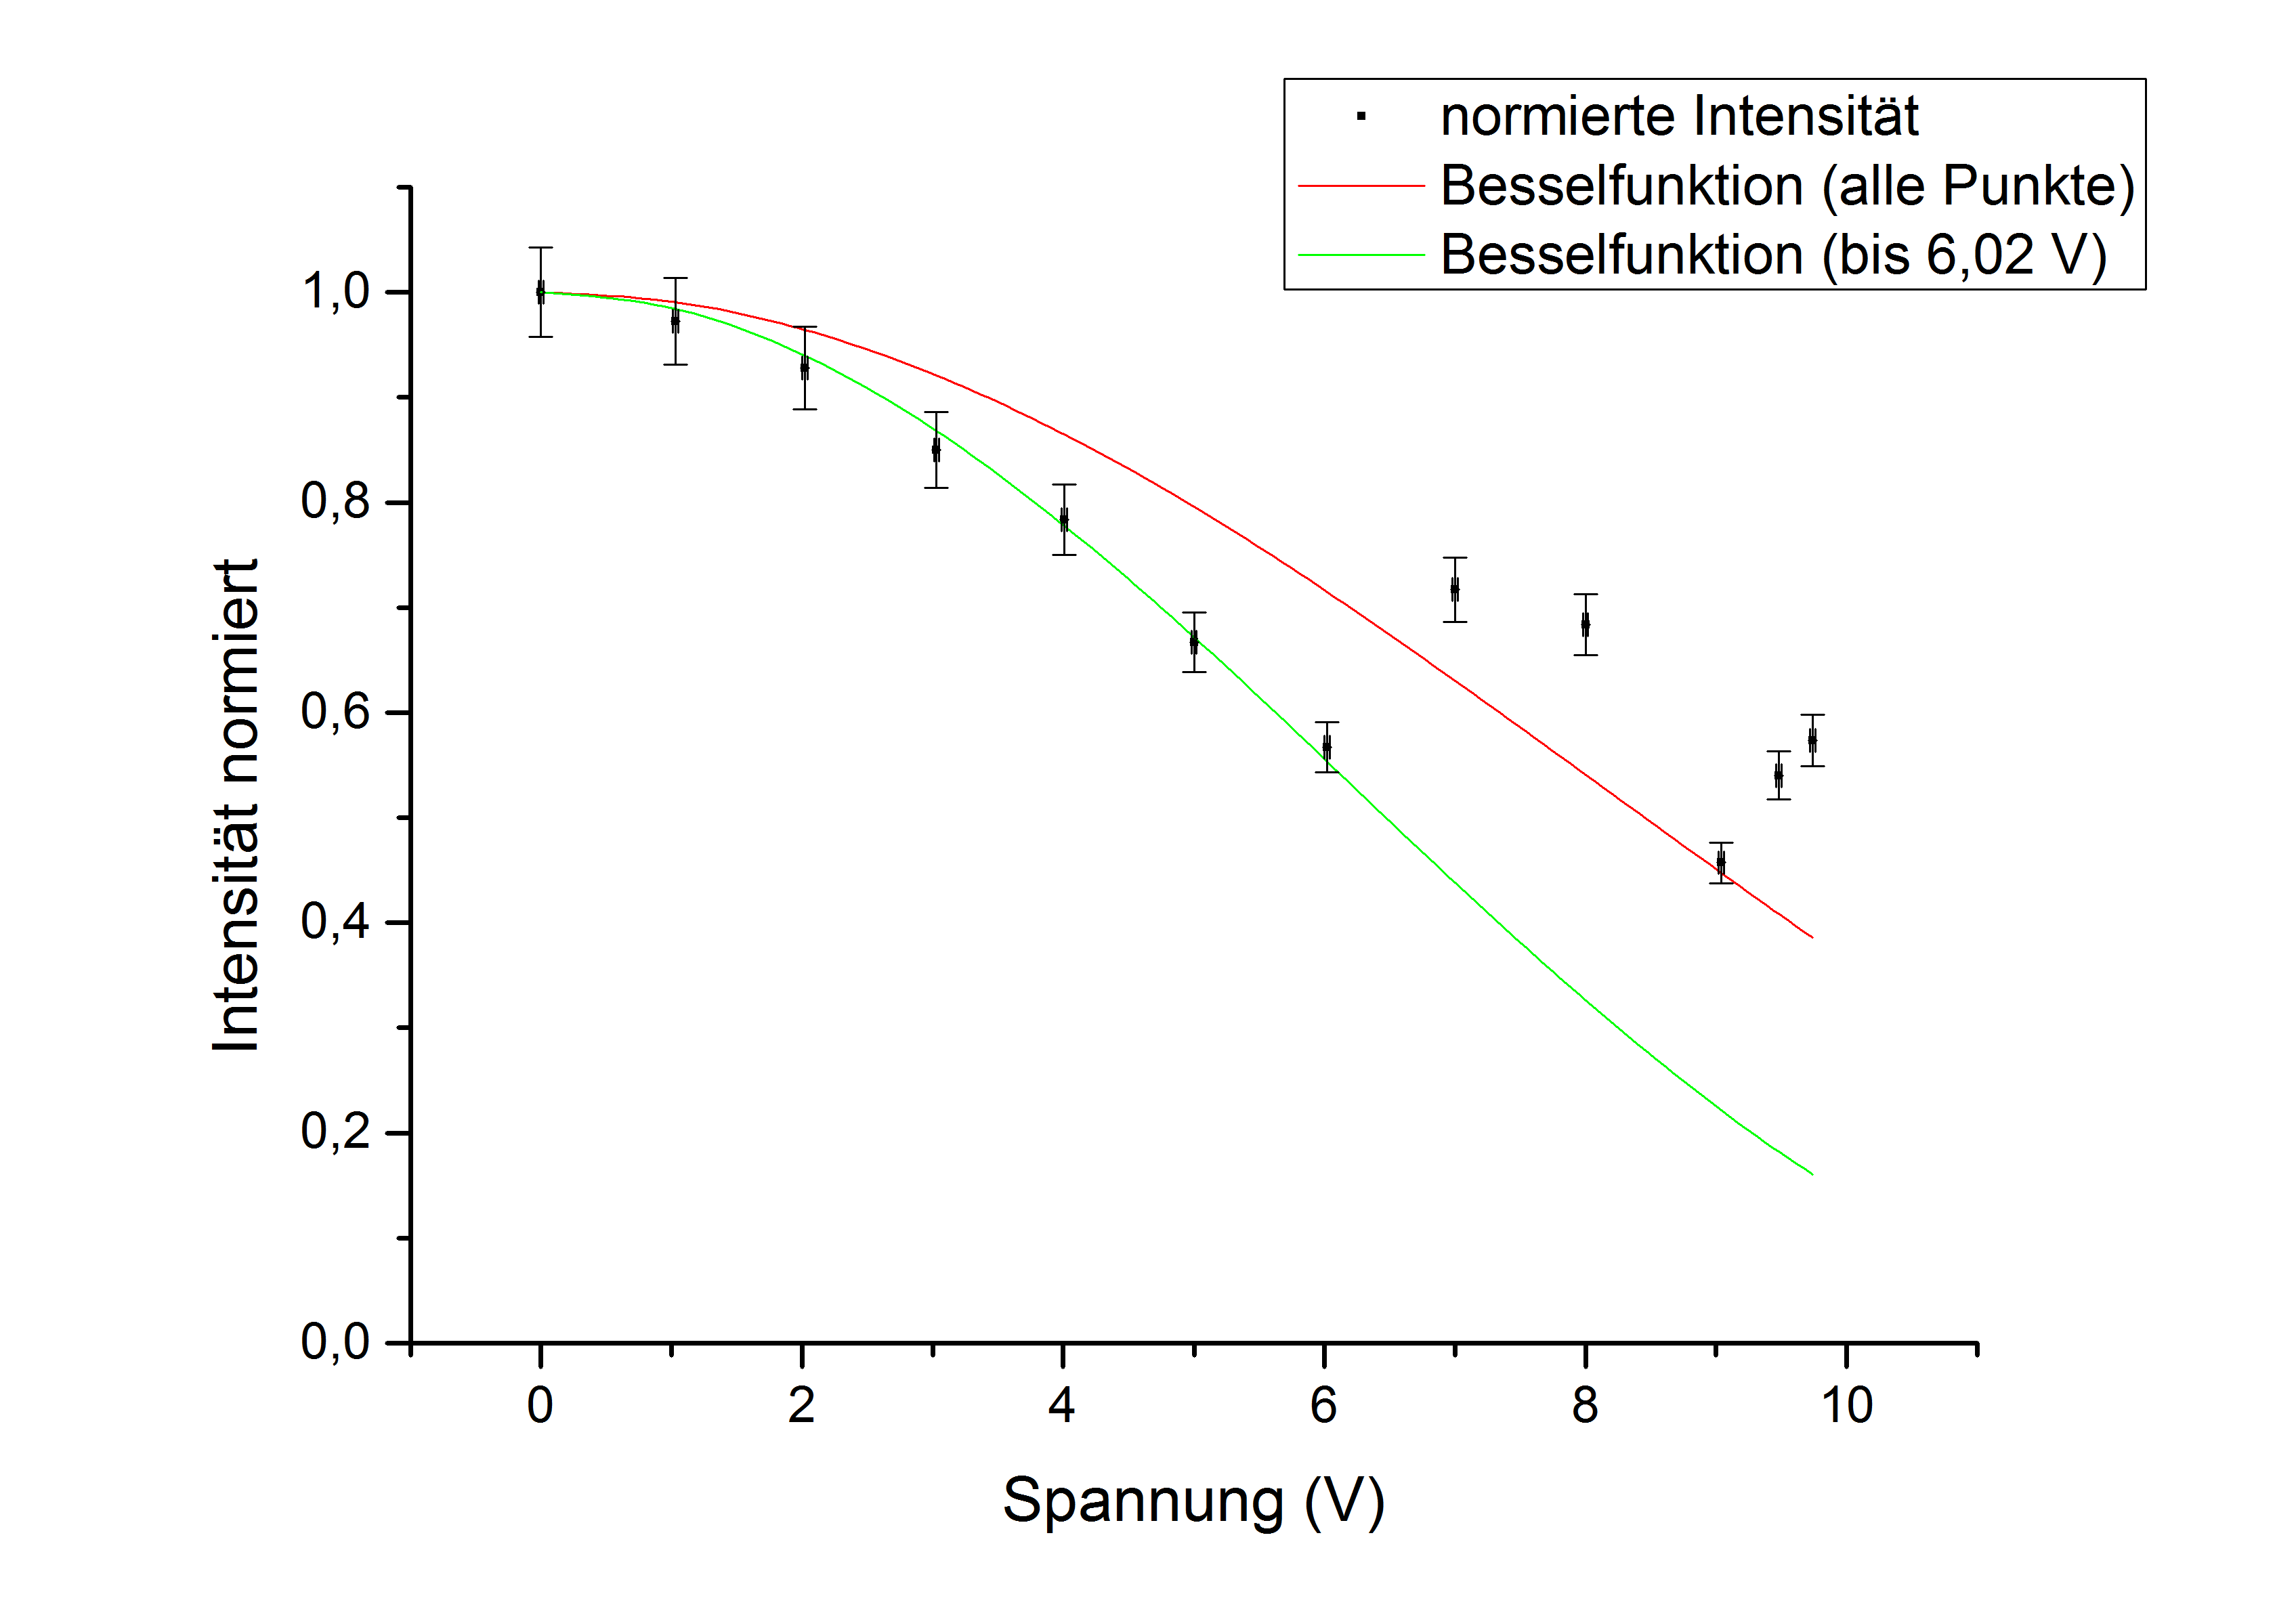
\includegraphics[scale=0.5]{Bilder/bessli0}
\caption{Vergleich 0. Beugungsordnung mit $J_{0}^{2}$}
\end{figure}
\end{center}
\clearpage
Wir verwendeten nicht die Methode, nach welcher der x-Wert des ersten Minimums der Besselfunktion $J_{0}(x)^{2}$ durch den x-Wert des Minimums der Intensität geteilt werden soll, um einen Umrechnungsfaktor zu bestimmen, da das Minimum der Besselfunktion bei 0 liegt und dieser Wert in unserem Verlauf bei den angelegten Spannungen nicht erreicht wird. Stattdessen fitteten wir eine quadratische Besselfunktion 0. Ordnung an unsere Punkte. Es ist gut zu sehen, dass für die ersten 7 Punkte (bis $6,02 V$) ein solcher Fit die gemessenen Punkte sehr gut beschreibt, die Theorie also bestätigt werden kann. Nimmt man nun aber auch die restlichen Werte hinzu, so sind Diskrepanzen zwischen dem theoretischen Verlauf und den tatsächlich vermessenen Werten zu beobachten. Dies kann an einer Erwärmung des Isooktans liegen, welches, da wir die Messreihe zweimal aufnahmen, da im ersten Durchlauf manche Maxima nicht gut sichtbar waren, und in dieser Messreihe für jede Ordnung ein eigenes Bild erstellten, sehr lange einer angelegten Spannung ausgesetzt war. Da die Werte ab $7,00V$ als letzte aufgenommen wurden, ist bei diesen der Effekt am größten. Betrachtet man aber die große Abweichung von dem theoretischen Verlauf, welcher die ersten 7 Punkte beschreibt, so wird die Vermutung nahegelegt, dass hierbei das Problem vielmehr bei den während der Messung beobachteten Schwankungen des Beugungsbildes bestand. Bei kleinen Modifizierungen der anliegenden Frequenz änderte sich das entstehende Bild teilweise drastisch.\\
\begin{center}
\begin{figure}[htbp]
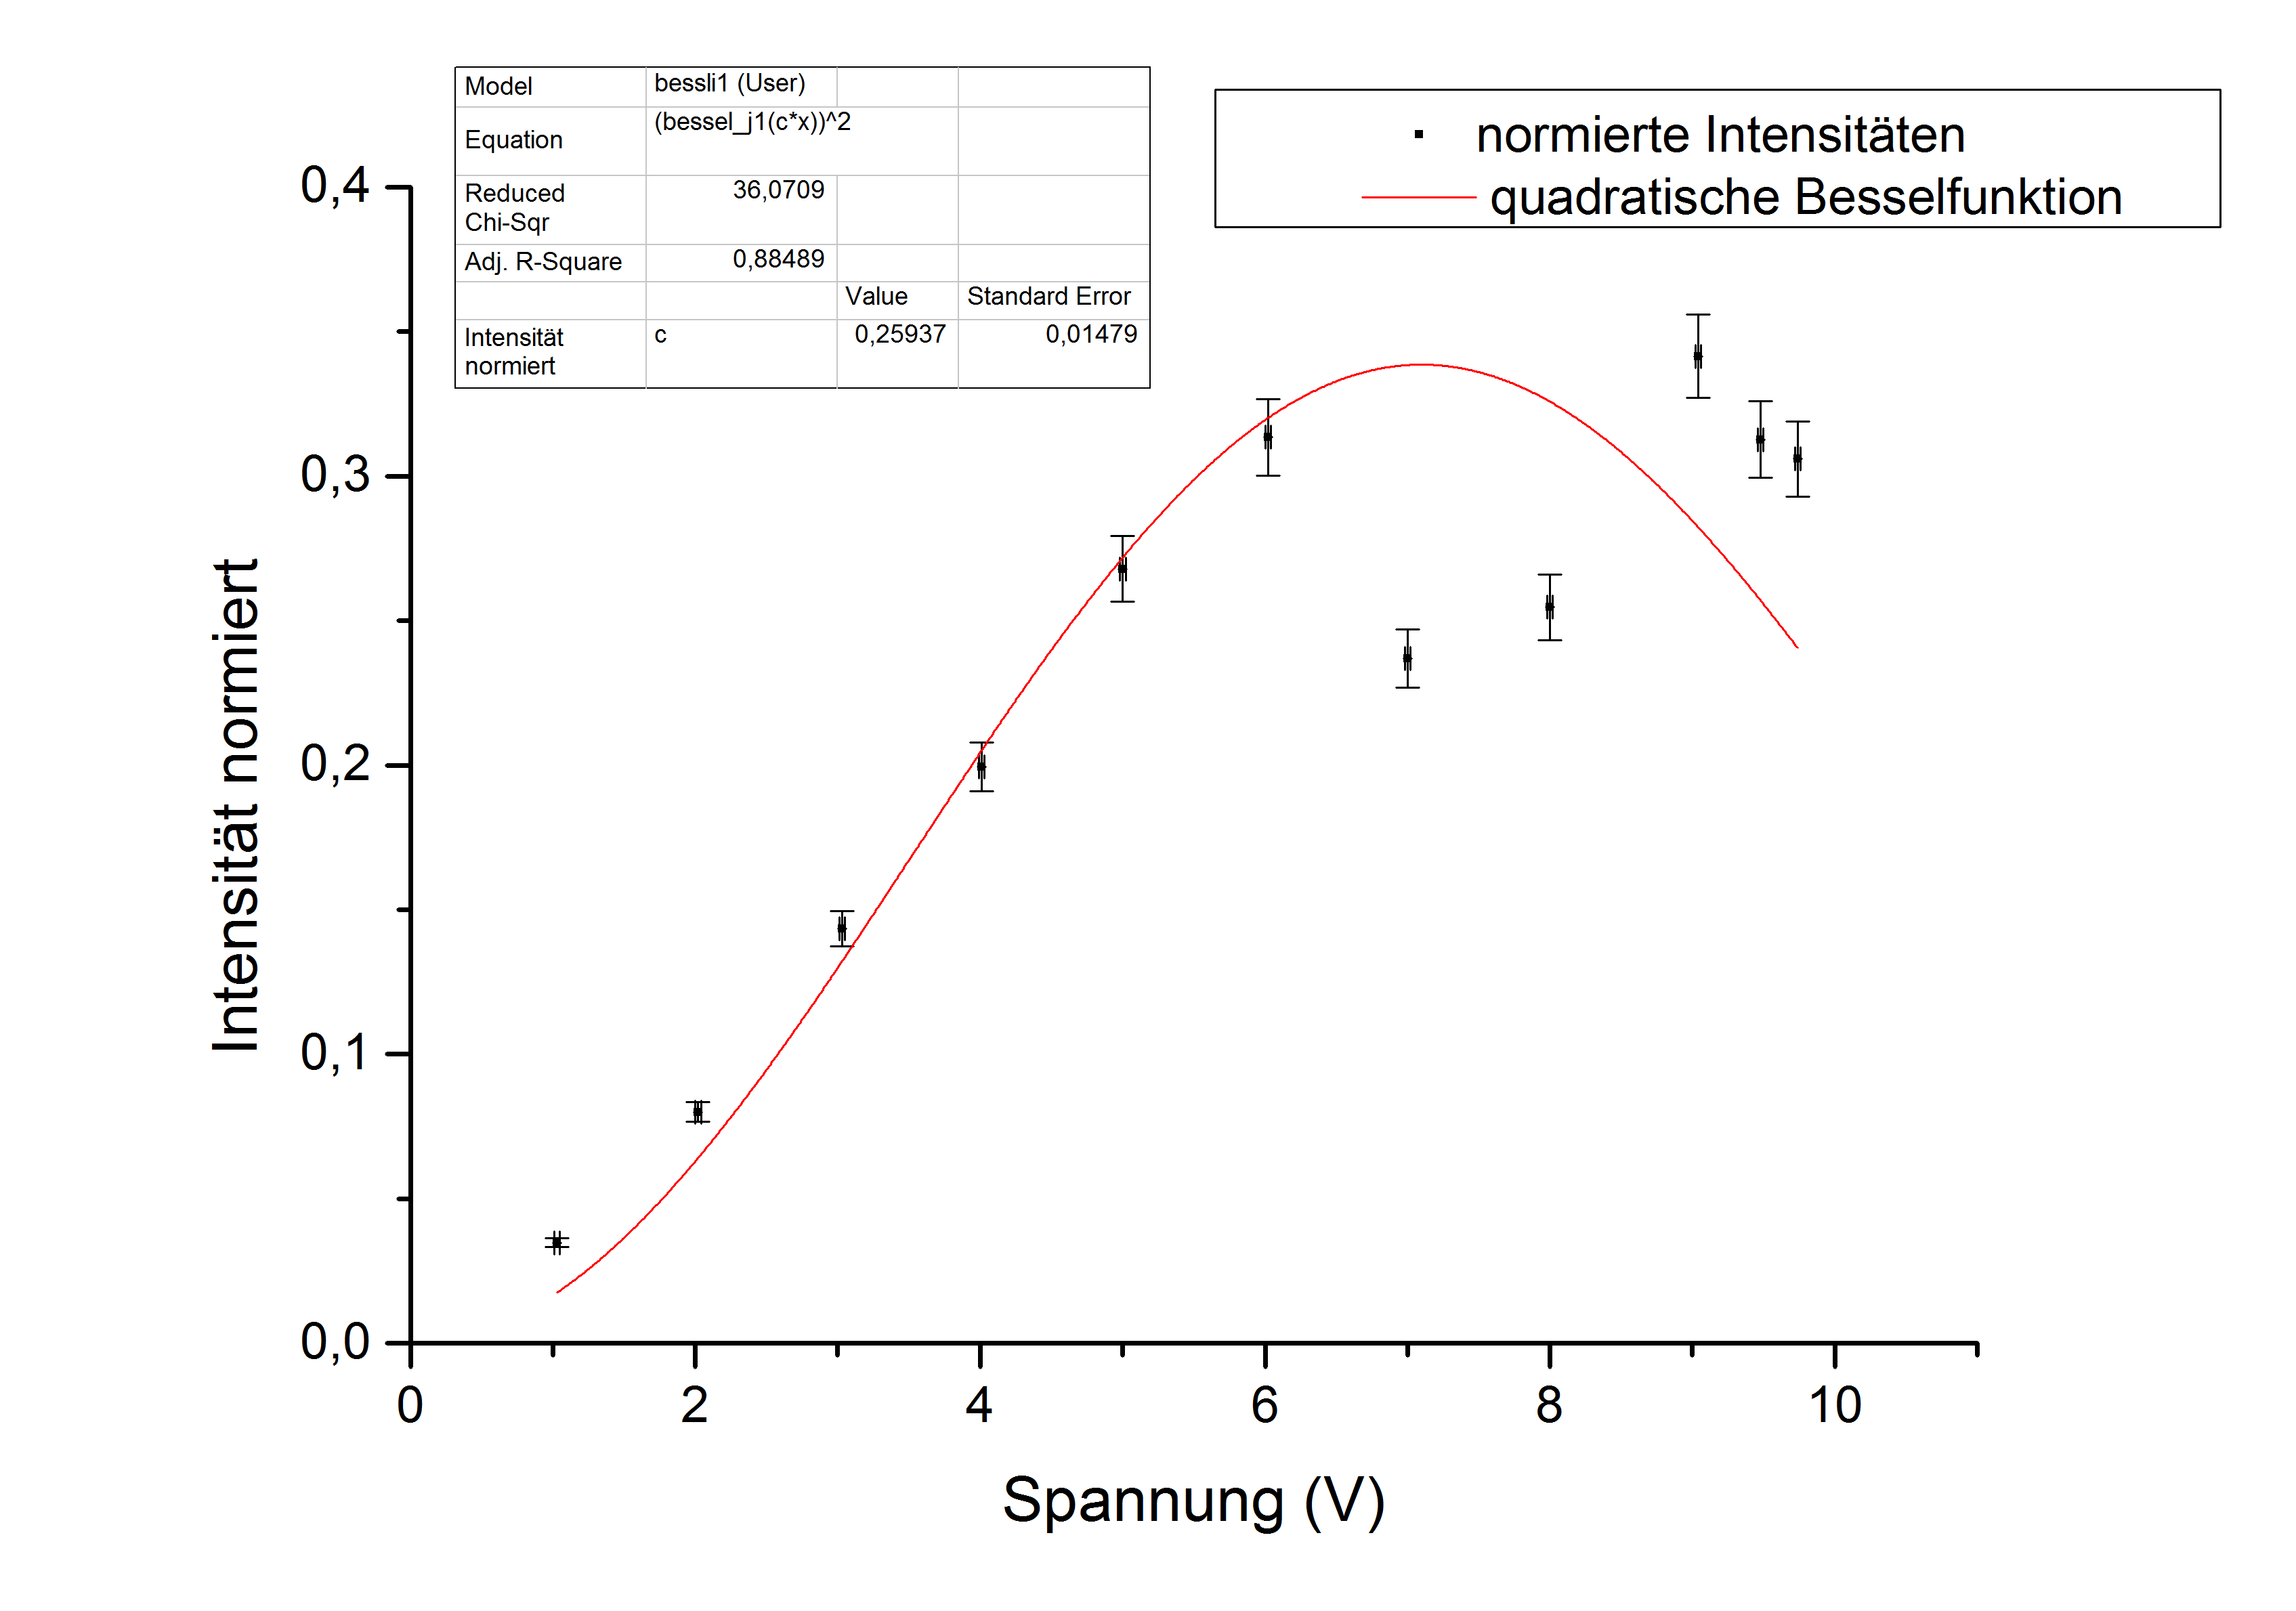
\includegraphics[scale=0.5]{Bilder/bessel1}
\caption{Vergleich 1. Beugungsordnung mit $J_{1}^{2}$}
\end{figure}
\end{center}
Für die 1. Beugungsordnung gilt das bereits für die 0. Ordnung erwähnte: Für die Werte bis $6,02 V$ ist der theoretische Verlauf gut zu bestätigen, für die Werte mit größerer Spannung ist die Streuung wesentlich größer.\\
\begin{center}
\begin{figure}[htbp]
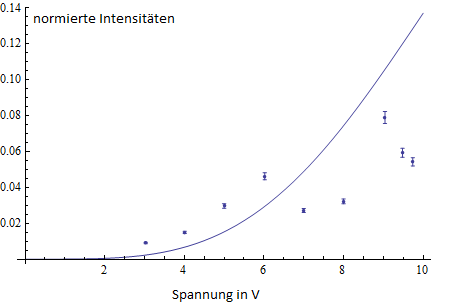
\includegraphics[scale=0.9]{Bilder/bessel2korr}
\caption{Vergleich 2. Beugungsordnung mit $J_{2}^{2}$}
\end{figure}
\end{center}
\begin{center}
\begin{figure}[htbp]
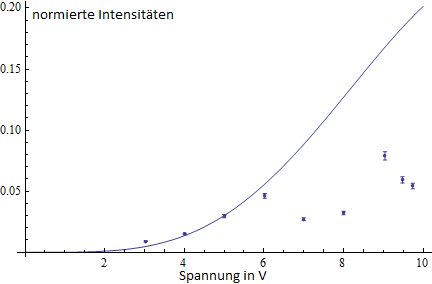
\includegraphics[scale=0.9]{Bilder/bessel21korr}
\caption{Vergleich 2. Beugungsordnung mit $J_{2}^{2}$ für Werte bis $6,02V$}
\end{figure}
\end{center}
Auch für die Werte der 2. Beugungsordnung können die Werte bis $6,02V$ gut durch eine quadratische Besselfunktion der entsprechenden Ordnung angenähert werden. Für den kompletten Verlauf gilt dies nicht. \\
Betrachtet man die Werte mit $U=7,00 V$ bzw. $U=8,00V$, so fällt auf, dass bei diesen der Peak der 0. Ordnung zu hoch, die Peaks der 1. und 2. Ordnung dagegen zu niedrig gemessen wurden. Dies ist genau der Effekt, der bei einer kleinen Variation der Frequenz zustande kam. Diesen Fehler konnten wir nicht verhindern, da wir bemüht waren, die Frequenz möglichst konstant zu lassen.\\
\subsubsection{Bestimmung der Schallwellenlänge}
Um die Schallwellenlänge $\Lambda$ zu bestimmen, benutzten wir Gitter 1, um mithilfe dieses Gitters die gemessenen Zeiten in Winkel transformieren zu können. Die Messwerte sind im Anhang zu finden. Der Fehler auf sie berechnet sich durch $s_{t}=0,03t$ (Quelle: [ham]). Um eine Ursprungsgerade zu erhalten, zogen wir von allen ausgelesenen Zeiten $t_{0}$ (die zur 0. Ordnung (m=0) korrespondierende Zeit) ab und trugen \[\sin(\theta)=\frac{m\lambda}{K}\] über diese auf (K steht hierbei für die Gitterkonstante des Gitters 1). Der Fehler auf diese Größe berechnet sich durch \[s_{\sin(\theta)}=\left|\sin(\theta)\right|\cdot\frac{s_{K}}{K}.\] Der resultierende lineare Fit sieht folgendermaßen aus:\\
\begin{center}
\begin{figure}[htbp]
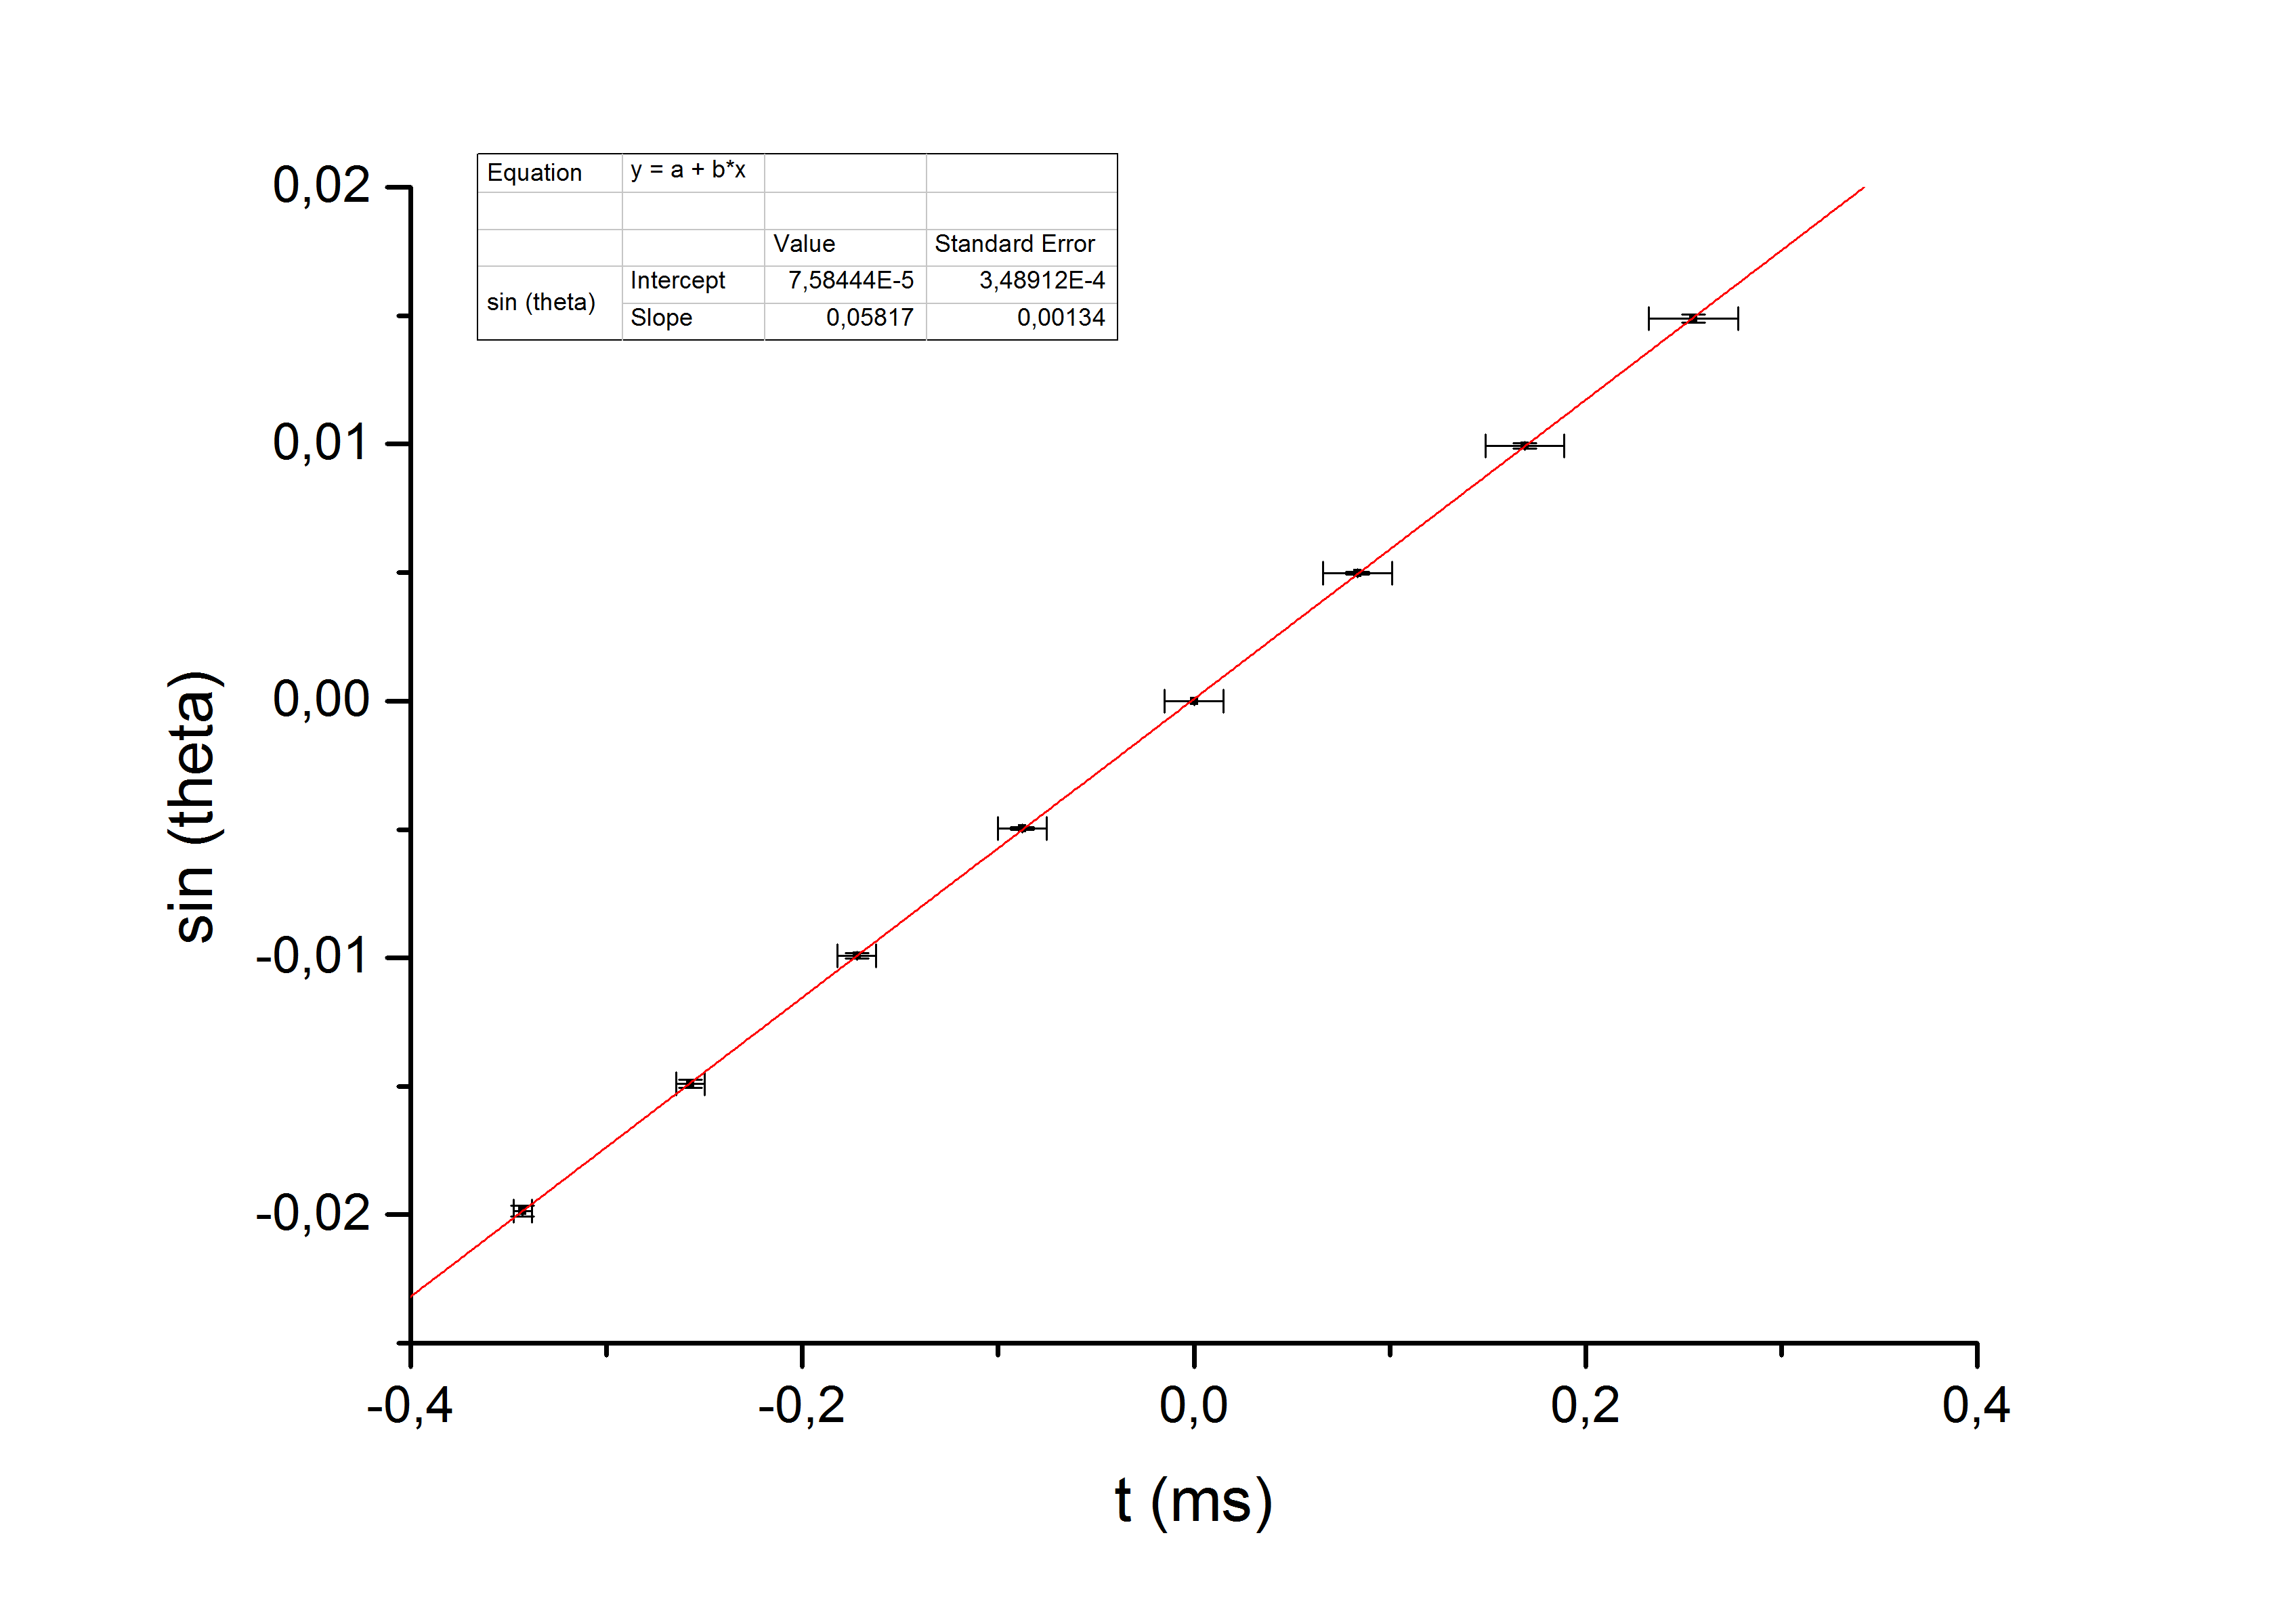
\includegraphics[scale=0.5]{Bilder/linfit}
\caption{Linearer Fit analog zu Aufgabe 2}
\end{figure}
\end{center}
Die Schallwellenlänge konnte nun bestimmt werden durch \[\Lambda=\frac{m\lambda}{at_{m}+b},\] wobei als Zeiten $t_{m}$ die mithilfe des Ultraschall-Phasengitters bestimmten Werte verwendet wurden (für die Messwerte s. Anhang). Dabei gilt \[t_{m}=t_{m_{gemessen}}-t_{0_{gemessen}},\] analog zu der Bestimmung der Zeiten für den linearen Fit. Der Fehler berechnet sich durch \[s_{t_{m}}=0,03\cdot s_{t_{m_{gemessen}}} (Quelle: [ham]).\] Somit erhalten wir $2m$ Werte für $\Lambda$ (für $m=0$ ergibt sich $\Lambda=0$: Dieser Wert wird vernachlässigt). Der Fehler berechnet sich mithilfe der Gauss'schen Fehlerfortpflanzung durch \[s_{\Lambda}=\left|\frac{m\lambda}{(at_{m}+b)^{2}}\right|\cdot\sqrt{(a\cdot s_{t_{m}})^{2}+(t_{m}\cdot s_{a})^{2}+s_{b}^{2}}.\] Den resultierenden Wert für die Schallwellenlänge erhielten wir durch gewichtete Mittelung: \[\bar{\Lambda}=(5,2\pm0,3)\cdot 10^{-4}m.\]Mithilfe der in der den Versuchsunterlagen beigefügten Staatsexamensarbeit gegebenen Schallgeschwindigkeit von $c_{iso}=1111 \frac{m}{s}$ erhält man eine Schallfrequenz von \[f=\frac{c_{iso}}{\Lambda}\] mit Fehler \[s_{f}=f\cdot\frac{s_{\Lambda}}{\Lambda}.\]
\[\Rightarrow f=(2,15\pm0,12)MHz\]
Dieser Wert stimmt im Rahmen der Messungenauigkeit mit der eingestellten Frequenz von $f_{ein}=2,1686MHz$ (s. Anhang) überein.